\documentclass{beamer}
\usepackage{listings}

\usepackage[skins]{tcolorbox}

\newcommand\blank[1]{\rule[-.2ex]{#1}{.4pt}}
\usepackage{tikz}
\usetikzlibrary{fit,backgrounds}
\usetikzlibrary{calc} % <-- important
\usetikzlibrary{decorations}
\usetikzlibrary{decorations.pathreplacing}

\usetikzlibrary{shapes.callouts, positioning, arrows.meta}

% Use plain theme with no decorations
\usetheme{default}
\setbeamertemplate{navigation symbols}{}
\setbeamertemplate{footline}{}
\setbeamertemplate{headline}{}

% Define Java code style
\lstdefinestyle{JavaStyle}{
    language=Java,
    basicstyle=\ttfamily\small,
    keywordstyle=\color{blue}\bfseries,
    commentstyle=\color{green!60!black},
    stringstyle=\color{orange},
    numbers=left,
    numberstyle=\tiny\color{gray},
    stepnumber=1,
    numbersep=10pt,
    breaklines=true,
    frame=single,
    tabsize=2,
    showstringspaces=false
}

\title{Exemple: La représentation binaire d'un nombre à virgule flottante\newline}
\subtitle{Algorithmes et Pensée Computationelle}
\author{École des Sciences Criminelles - UNIL}
\date{}

\begin{document}

\begin{frame}
\titlepage
\end{frame}

\begin{frame}
Voici la représentation en binaire d'un nombre à virgule flottante: 
\begin{table}[h]
\centering
\renewcommand{\arraystretch}{1.3}
\begin{tabular}{|c|c|c|}
\hline
\textbf{Signe} & \textbf{Exposant (8 bits)} & \textbf{Mantissa (23 bits)} \\
\hline
1 & 10001000 & 01000100000000000001000 \\
\hline
\end{tabular}
\end{table}
Que vaut cette représentation en base 10? Utiliser la représentation des floating points (avec un biais de 127). Arrondir les résultats intermédiaires et la valeur finale au 7ème chiffre significatif après la virgule.

\end{frame}
\begin{frame}[fragile]{Calcul du $1+\displaystyle \Sigma_{i=1}^{23} b_{23-i}2^{-i}$}

\begin{tcolorbox}
\begin{block}{Rappel}
\small
$\Sigma_{i=1}^{n} x_i = x_1 + x_2 + x_3 + .. + x_n$
\end{block}
\end{tcolorbox}

\begin{center}
\resizebox{\textwidth}{!}{
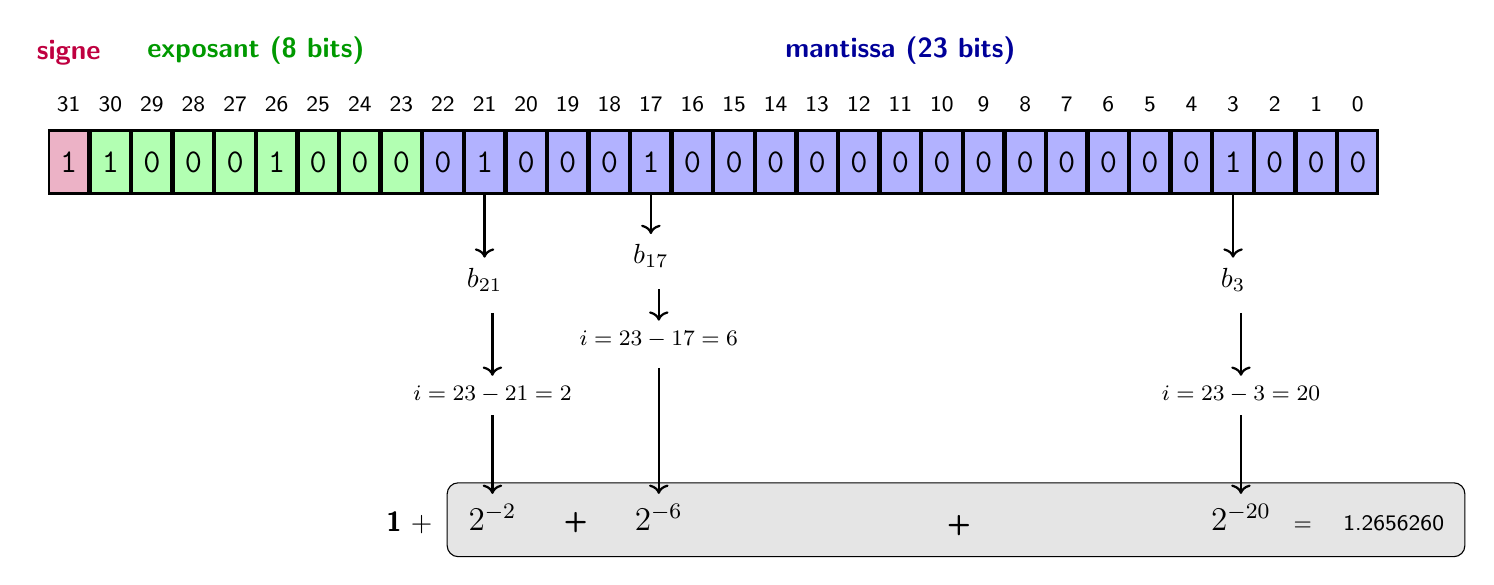
\begin{tikzpicture}[font=\sffamily]
% Box styles
\tikzset{
  bit/.style={minimum width=0.5cm, minimum height=0.8cm, draw=black, thick, font=\ttfamily\large},
  sign/.style={fill=purple!30},
  exponent/.style={fill=green!30},
  mantissa/.style={fill=blue!30},
  bigbit/.style={minimum width=1.0cm, minimum height=1.2cm, draw=black, very thick, font=\ttfamily\Large}
}

% Sign bit
\node[bit,sign] (b31) {1};

% Exponent bits (8)
\node[bit,exponent,right=0cm of b31] (b30) {1};
\node[bit,exponent,right=0cm of b30] (b29) {0};
\node[bit,exponent,right=0cm of b29] (b28) {0};
\node[bit,exponent,right=0cm of b28] (b27) {0};
\node[bit,exponent,right=0cm of b27] (b26) {1};
\node[bit,exponent,right=0cm of b26] (b25) {0};
\node[bit,exponent,right=0cm of b25] (b24) {0};
\node[bit,exponent,right=0cm of b24] (b23) {0};

% Mantissa bits (23)
\node[bit,mantissa,right=0cm of b23] (b22) {0};
\node[bit,mantissa,right=0cm of b22] (b21) {1};
\node[bit,mantissa,right=0cm of b21] (b20) {0};
\node[bit,mantissa,right=0cm of b20] (b19) {0};
\node[bit,mantissa,right=0cm of b19] (b18) {0};
\node[bit,mantissa,right=0cm of b18] (b17) {1};
\node[bit,mantissa,right=0cm of b17] (b16) {0};
\node[bit,mantissa,right=0cm of b16] (b15) {0};
\node[bit,mantissa,right=0cm of b15] (b14) {0};
\node[bit,mantissa,right=0cm of b14] (b13) {0};
\node[bit,mantissa,right=0cm of b13] (b12) {0};
\node[bit,mantissa,right=0cm of b12] (b11) {0};
\node[bit,mantissa,right=0cm of b11] (b10) {0};
\node[bit,mantissa,right=0cm of b10] (b9)  {0};
\node[bit,mantissa,right=0cm of b9]  (b8)  {0};
\node[bit,mantissa,right=0cm of b8]  (b7)  {0};
\node[bit,mantissa,right=0cm of b7]  (b6)  {0};
\node[bit,mantissa,right=0cm of b6]  (b5)  {0};
\node[bit,mantissa,right=0cm of b5]  (b4)  {0};
\node[bit,mantissa,right=0cm of b4]  (b3)  {1};
\node[bit,mantissa,right=0cm of b3]  (b2)  {0};
\node[bit,mantissa,right=0cm of b2]  (b1)  {0};
\node[bit,mantissa,right=0cm of b1]  (b0)  {0};

% Labels under each bit
\node[above=0.1cm of b31] {\footnotesize 31};
\node[above=0.1cm of b30] {\footnotesize 30};
\node[above=0.1cm of b29] {\footnotesize 29};
\node[above=0.1cm of b28] {\footnotesize 28};
\node[above=0.1cm of b27] {\footnotesize 27};
\node[above=0.1cm of b26] {\footnotesize 26};
\node[above=0.1cm of b25] {\footnotesize 25};
\node[above=0.1cm of b24] {\footnotesize 24};
\node[above=0.1cm of b23] {\footnotesize 23};
\node[above=0.1cm of b22] {\footnotesize 22};
\node[above=0.1cm of b21] {\footnotesize 21};
\node[above=0.1cm of b20] {\footnotesize 20};
\node[above=0.1cm of b19] {\footnotesize 19};
\node[above=0.1cm of b18] {\footnotesize 18};
\node[above=0.1cm of b17] {\footnotesize 17};
\node[above=0.1cm of b16] {\footnotesize 16};
\node[above=0.1cm of b15] {\footnotesize 15};
\node[above=0.1cm of b14] {\footnotesize 14};
\node[above=0.1cm of b13] {\footnotesize 13};
\node[above=0.1cm of b12] {\footnotesize 12};
\node[above=0.1cm of b11] {\footnotesize 11};
\node[above=0.1cm of b10] {\footnotesize 10};
\node[above=0.1cm of b9]  {\footnotesize 9};
\node[above=0.1cm of b8]  {\footnotesize 8};
\node[above=0.1cm of b7]  {\footnotesize 7};
\node[above=0.1cm of b6]  {\footnotesize 6};
\node[above=0.1cm of b5]  {\footnotesize 5};
\node[above=0.1cm of b4]  {\footnotesize 4};
\node[above=0.1cm of b3]  {\footnotesize 3};
\node[above=0.1cm of b2]  {\footnotesize 2};
\node[above=0.1cm of b1]  {\footnotesize 1};
\node[above=0.1cm of b0]  {\footnotesize 0};

% Arrow pointing down from bits which are 1 in the mantissa
\draw[->, thick] (b17.south) -- ++(0,-0.5) node[below] {$b_{17}$};
\draw[->, thick] (b21.south) -- ++(0,-0.8) node[below] {$b_{21}$};
\draw[->, thick] (b3.south) -- ++(0,-0.8) node[below] {$b_3$};
%\draw[->, thick] (b5.south) -- ++(0,-0.8) node[below] {$b_5$};


% Arrow pointing down from bits which are 1 in the mantissa
% \draw[->, thick] (b9.south) -- ++(0,-0.8) node[below] {$b_9$};
% \draw[->, thick] (b21.south) -- ++(0,-0.8) node[below] {$b_{21}$};
% \draw[->, thick] (b3.south) -- ++(0,-0.8) node[below] {$b_3$};
% \draw[->, thick] (b5.south) -- ++(0,-0.8) node[below] {$b_5$};


%draw the i's
\draw[->, thick] (b17.south) ++(0.1,-1.2) -- ++(0,-0.4) node[below] {\footnotesize $i=23-17=6$};
\draw[->, thick] (b21.south) ++(0.1,-1.5) -- ++(0,-0.8) node[below] {\footnotesize $i=23-21=2$};
\draw[->, thick] (b3.south) ++(0.1,-1.5) -- ++(0,-0.8) node[below] {\footnotesize $i=23-3=20$};

%draw the powers of 2

% \draw[->, thick] (b17.south) ++(0.1,-2.8) -- ++(0,-0.8) node[below] {\footnotesize $2^{-6}$};
% \draw[->, thick] (b3.south) ++(0.1,-2.8) -- ++(0,-0.8) node[below] {\footnotesize $2^{-20}$};
% \draw[->, thick] (b21.south) ++(0.1,-2.8) -- ++(0,-0.8) node[below] {\footnotesize $2^{-2}$};

%your three arrow+nodes
\draw[->, thick] (b17.south) ++(0.1,-2.2) -- ++(0,-1.6)
    node[below] (n14) {\large $2^{-6}$};

\draw[->, thick] (b3.south) ++(0.1,-2.8) -- ++(0,-1)
    node[below] (n20) {\large $2^{-20}$};

\draw[->, thick] (b21.south) ++(0.1,-2.8) -- ++(0,-1)
    node[below] (n2) {\large $2^{-2}$};

% midpoint coordinate
\path let \p1 = (n14), \p2 = (n20) in 
      coordinate (mid) at ($(\p1)!.5!(\p2)$);

\path let \p1 = (n2), \p2 = (n14) in 
      coordinate (mid2) at ($(\p1)!.5!(\p2)$);

% place a plus sign there
\node[yshift=-2pt] at (mid2) {$\textbf{+}$};
%\node[yshift=-2pt] at (mid) {$\textbf{+}$};
\node[xshift=-30pt, yshift=-2pt] at (n2) {$\textbf{1} \ +$};


\node[xshift=0pt, yshift=-3pt] (eq) at (mid) {\ \ $\textbf{+}$};
\node[xshift=150pt, yshift=-2pt] (n20) at (mid) {\footnotesize $\shortstack{\ = \ \ \   1.2656260}$};


% put the rectangle behind
\begin{pgfonlayer}{background}
  \node[draw, fill=gray!20, rounded corners,
        fit=(n20)(eq)(n2), inner sep=4pt, yshift=0pt] {};
\end{pgfonlayer}



% Braces and labels
\draw[decorate,decoration={mirror,amplitude=5pt}] (b31.north west) -- (b31.north east) node[midway,above=0.7cm,black]{\textcolor{purple}{\textbf{signe}}};

\draw[decorate,decoration={amplitude=5pt}] (b30.north west) -- (b23.north east) node[midway,above=0.7cm,black]{\textcolor{green!60!black}{\textbf{exposant (8 bits)}}};

\draw[decorate,decoration={amplitude=5pt}] (b22.north west) -- (b0.north east) node[midway,above=0.7cm,black]{\textcolor{blue!60!black}{\textbf{mantissa (23 bits)}}};

\end{tikzpicture}
}
\end{center}
\end{frame}

\begin{frame}[fragile]{Calcul de l'exposant $2^{e-127}$}
\begin{center}
\resizebox{\textwidth}{!}{
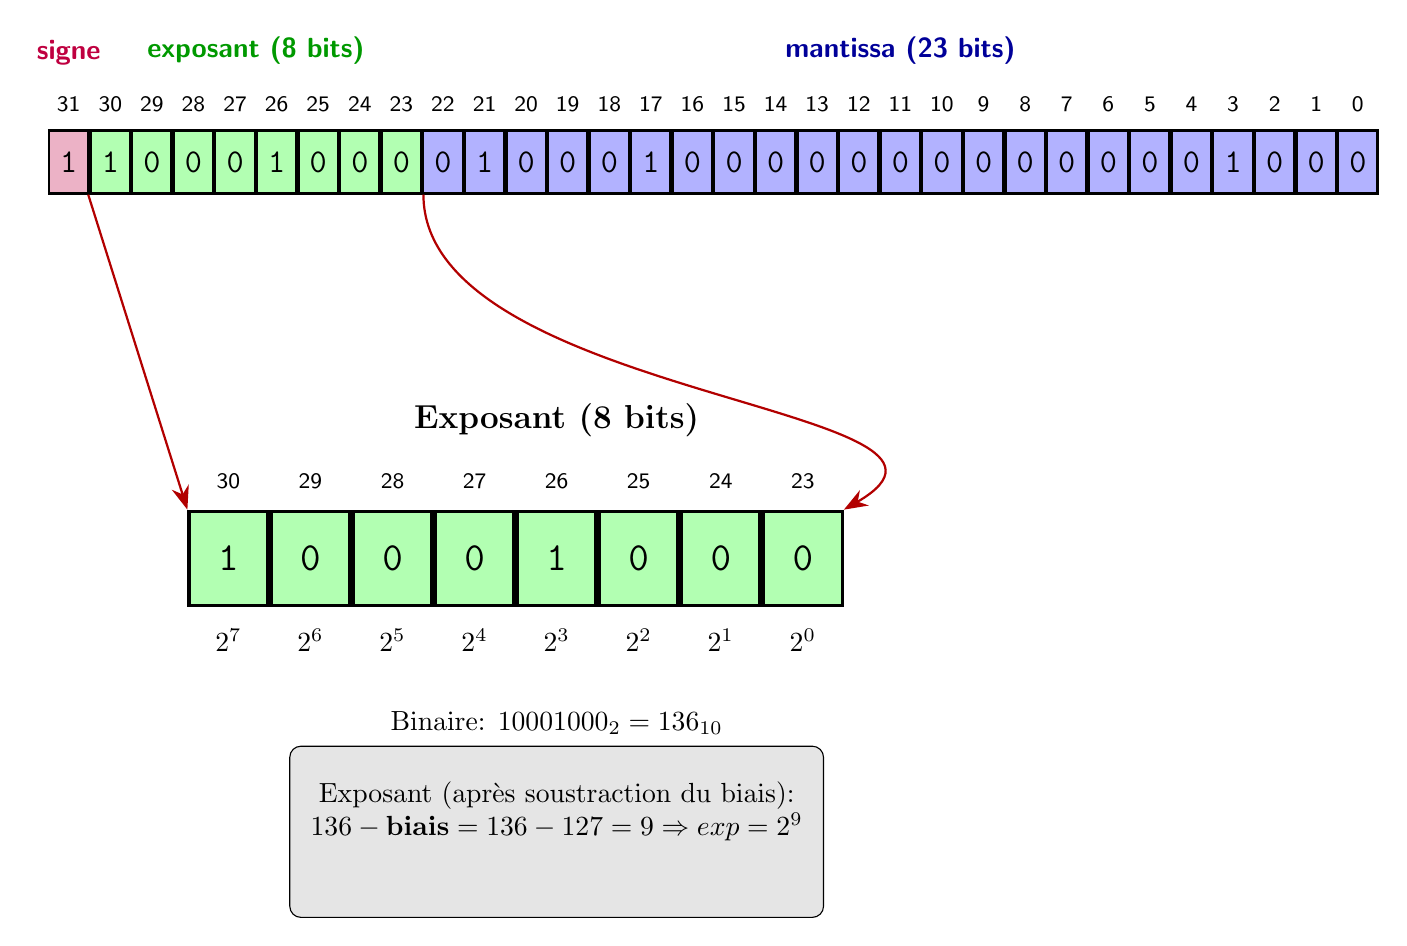
\begin{tikzpicture}[font=\sffamily]
% Box styles
\tikzset{
  bit/.style={minimum width=0.5cm, minimum height=0.8cm, draw=black, thick, font=\ttfamily\large},
  sign/.style={fill=purple!30},
  exponent/.style={fill=green!30},
  mantissa/.style={fill=blue!30},
  bigbit/.style={minimum width=1.0cm, minimum height=1.2cm, draw=black, very thick, font=\ttfamily\Large}
}

% Sign bit
\node[bit,sign] (b31) {1};

% Exponent bits (8)
\node[bit,exponent,right=0cm of b31] (b30) {1};
\node[bit,exponent,right=0cm of b30] (b29) {0};
\node[bit,exponent,right=0cm of b29] (b28) {0};
\node[bit,exponent,right=0cm of b28] (b27) {0};
\node[bit,exponent,right=0cm of b27] (b26) {1};
\node[bit,exponent,right=0cm of b26] (b25) {0};
\node[bit,exponent,right=0cm of b25] (b24) {0};
\node[bit,exponent,right=0cm of b24] (b23) {0};

% Mantissa bits (23)
\node[bit,mantissa,right=0cm of b23] (b22) {0};
\node[bit,mantissa,right=0cm of b22] (b21) {1};
\node[bit,mantissa,right=0cm of b21] (b20) {0};
\node[bit,mantissa,right=0cm of b20] (b19) {0};
\node[bit,mantissa,right=0cm of b19] (b18) {0};
\node[bit,mantissa,right=0cm of b18] (b17) {1};
\node[bit,mantissa,right=0cm of b17] (b16) {0};
\node[bit,mantissa,right=0cm of b16] (b15) {0};
\node[bit,mantissa,right=0cm of b15] (b14) {0};
\node[bit,mantissa,right=0cm of b14] (b13) {0};
\node[bit,mantissa,right=0cm of b13] (b12) {0};
\node[bit,mantissa,right=0cm of b12] (b11) {0};
\node[bit,mantissa,right=0cm of b11] (b10) {0};
\node[bit,mantissa,right=0cm of b10] (b9)  {0};
\node[bit,mantissa,right=0cm of b9]  (b8)  {0};
\node[bit,mantissa,right=0cm of b8]  (b7)  {0};
\node[bit,mantissa,right=0cm of b7]  (b6)  {0};
\node[bit,mantissa,right=0cm of b6]  (b5)  {0};
\node[bit,mantissa,right=0cm of b5]  (b4)  {0};
\node[bit,mantissa,right=0cm of b4]  (b3)  {1};
\node[bit,mantissa,right=0cm of b3]  (b2)  {0};
\node[bit,mantissa,right=0cm of b2]  (b1)  {0};
\node[bit,mantissa,right=0cm of b1]  (b0)  {0};

% Labels under each bit
\node[above=0.1cm of b31] {\footnotesize 31};
\node[above=0.1cm of b30] {\footnotesize 30};
\node[above=0.1cm of b29] {\footnotesize 29};
\node[above=0.1cm of b28] {\footnotesize 28};
\node[above=0.1cm of b27] {\footnotesize 27};
\node[above=0.1cm of b26] {\footnotesize 26};
\node[above=0.1cm of b25] {\footnotesize 25};
\node[above=0.1cm of b24] {\footnotesize 24};
\node[above=0.1cm of b23] {\footnotesize 23};
\node[above=0.1cm of b22] {\footnotesize 22};
\node[above=0.1cm of b21] {\footnotesize 21};
\node[above=0.1cm of b20] {\footnotesize 20};
\node[above=0.1cm of b19] {\footnotesize 19};
\node[above=0.1cm of b18] {\footnotesize 18};
\node[above=0.1cm of b17] {\footnotesize 17};
\node[above=0.1cm of b16] {\footnotesize 16};
\node[above=0.1cm of b15] {\footnotesize 15};
\node[above=0.1cm of b14] {\footnotesize 14};
\node[above=0.1cm of b13] {\footnotesize 13};
\node[above=0.1cm of b12] {\footnotesize 12};
\node[above=0.1cm of b11] {\footnotesize 11};
\node[above=0.1cm of b10] {\footnotesize 10};
\node[above=0.1cm of b9]  {\footnotesize 9};
\node[above=0.1cm of b8]  {\footnotesize 8};
\node[above=0.1cm of b7]  {\footnotesize 7};
\node[above=0.1cm of b6]  {\footnotesize 6};
\node[above=0.1cm of b5]  {\footnotesize 5};
\node[above=0.1cm of b4]  {\footnotesize 4};
\node[above=0.1cm of b3]  {\footnotesize 3};
\node[above=0.1cm of b2]  {\footnotesize 2};
\node[above=0.1cm of b1]  {\footnotesize 1};
\node[above=0.1cm of b0]  {\footnotesize 0};


% Invisible node to mark exponent region
\node[fit=(b30)(b23), inner sep=0pt] (exp-region) {};

% Zoomed exponent bits below
\node[bigbit,exponent, below=4cm of b30, xshift=1.5cm] (z30) {1};
\node[bigbit,exponent,right=0cm of z30] (z29) {0};
\node[bigbit,exponent,right=0cm of z29] (z28) {0};
\node[bigbit,exponent,right=0cm of z28] (z27) {0};
\node[bigbit,exponent,right=0cm of z27] (z26) {1};
\node[bigbit,exponent,right=0cm of z26] (z25) {0};
\node[bigbit,exponent,right=0cm of z25] (z24) {0};
\node[bigbit,exponent,right=0cm of z24] (z23) {0};

% Bit position labels above zoomed bits
\node[above=0.15cm of z30] {\footnotesize 30};
\node[above=0.15cm of z29] {\footnotesize 29};
\node[above=0.15cm of z28] {\footnotesize 28};
\node[above=0.15cm of z27] {\footnotesize 27};
\node[above=0.15cm of z26] {\footnotesize 26};
\node[above=0.15cm of z25] {\footnotesize 25};
\node[above=0.15cm of z24] {\footnotesize 24};
\node[above=0.15cm of z23] {\footnotesize 23};

% Power of 2 labels below zoomed bits
\node[below=0.15cm of z30] {$2^7$};
\node[below=0.15cm of z29] {$2^6$};
\node[below=0.15cm of z28] {$2^5$};
\node[below=0.15cm of z27] {$2^4$};
\node[below=0.15cm of z26] {$2^3$};
\node[below=0.15cm of z25] {$2^2$};
\node[below=0.15cm of z24] {$2^1$};
\node[below=0.15cm of z23] {$2^0$};

% Title for zoomed section
\node[above=0.8cm of z26, font=\large\bfseries] {Exposant (8 bits)};

% Calculation annotation
\node[below=1.2cm of z26, font=\normalsize, align=center] (exp) {
Binaire: $10001000_2 = 136_{10}$ \\[0.2em]
\\Exposant (après soustraction du biais):\\ $136 - \textbf{biais} = 136 - 127 = 9 \Rightarrow exp = 2^9$
};

% put the rectangle behind
\begin{pgfonlayer}{background}
  \node[draw, fill=gray!20, rounded corners,
        fit=(exp), inner sep=4pt, yshift=-20pt] {};
\end{pgfonlayer}

% Arrows connecting original to zoomed view
\draw[-{Stealth[length=3mm]}, thick, red!70!black] (b30.south) ++(-0.28,0) -- (z30.north west);
\draw[-{Stealth[length=3mm]}, thick, red!70!black]
  (b23.south) ++(0.28,0)
  to[out=-90, in=30] (z23.north east);






Braces and labels
\draw[decorate,decoration={mirror,amplitude=5pt}] (b31.north west) -- (b31.north east) node[midway,above=0.7cm,black]{\textcolor{purple}{\textbf{signe}}};

\draw[decorate,decoration={amplitude=5pt}] (b30.north west) -- (b23.north east) node[midway,above=0.7cm,black]{\textcolor{green!60!black}{\textbf{exposant (8 bits)}}};

\draw[decorate,decoration={amplitude=5pt}] (b22.north west) -- (b0.north east) node[midway,above=0.7cm,black]{\textcolor{blue!60!black}{\textbf{mantissa (23 bits)}}};
\end{tikzpicture}
}
\end{center}
\end{frame}

\begin{frame}[fragile]{Calcul du signe $(-1)^{b_{31}}$}
\begin{center}
\resizebox{\textwidth}{!}{
\hspace{-1.1cm}
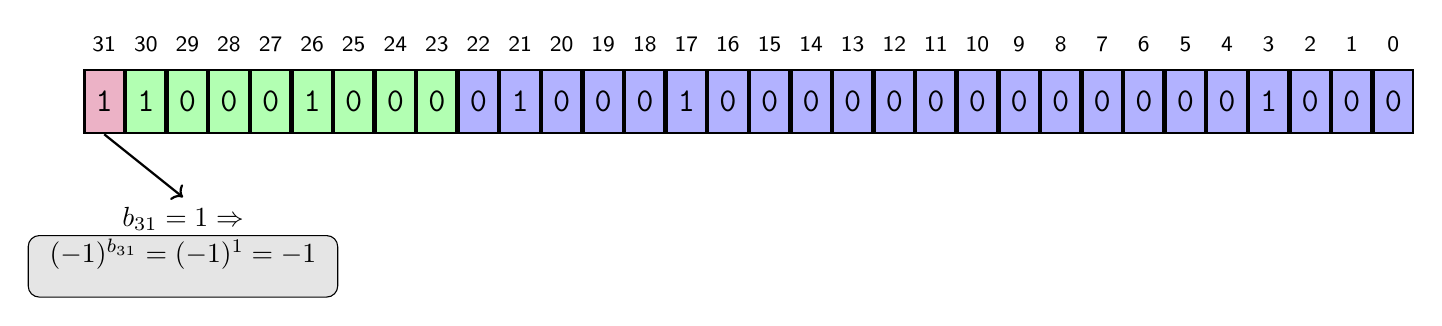
\begin{tikzpicture}[font=\sffamily]
% Box styles
\tikzset{
  bit/.style={minimum width=0.5cm, minimum height=0.8cm, draw=black, thick, font=\ttfamily\large},
  sign/.style={fill=purple!30},
  exponent/.style={fill=green!30},
  mantissa/.style={fill=blue!30},
  bigbit/.style={minimum width=1.0cm, minimum height=1.2cm, draw=black, very thick, font=\ttfamily\Large}
}

% Sign bit
\node[bit,sign] (b31) {1};

% Exponent bits (8)
\node[bit,exponent,right=0cm of b31] (b30) {1};
\node[bit,exponent,right=0cm of b30] (b29) {0};
\node[bit,exponent,right=0cm of b29] (b28) {0};
\node[bit,exponent,right=0cm of b28] (b27) {0};
\node[bit,exponent,right=0cm of b27] (b26) {1};
\node[bit,exponent,right=0cm of b26] (b25) {0};
\node[bit,exponent,right=0cm of b25] (b24) {0};
\node[bit,exponent,right=0cm of b24] (b23) {0};

% Mantissa bits (23)
\node[bit,mantissa,right=0cm of b23] (b22) {0};
\node[bit,mantissa,right=0cm of b22] (b21) {1};
\node[bit,mantissa,right=0cm of b21] (b20) {0};
\node[bit,mantissa,right=0cm of b20] (b19) {0};
\node[bit,mantissa,right=0cm of b19] (b18) {0};
\node[bit,mantissa,right=0cm of b18] (b17) {1};
\node[bit,mantissa,right=0cm of b17] (b16) {0};
\node[bit,mantissa,right=0cm of b16] (b15) {0};
\node[bit,mantissa,right=0cm of b15] (b14) {0};
\node[bit,mantissa,right=0cm of b14] (b13) {0};
\node[bit,mantissa,right=0cm of b13] (b12) {0};
\node[bit,mantissa,right=0cm of b12] (b11) {0};
\node[bit,mantissa,right=0cm of b11] (b10) {0};
\node[bit,mantissa,right=0cm of b10] (b9)  {0};
\node[bit,mantissa,right=0cm of b9]  (b8)  {0};
\node[bit,mantissa,right=0cm of b8]  (b7)  {0};
\node[bit,mantissa,right=0cm of b7]  (b6)  {0};
\node[bit,mantissa,right=0cm of b6]  (b5)  {0};
\node[bit,mantissa,right=0cm of b5]  (b4)  {0};
\node[bit,mantissa,right=0cm of b4]  (b3)  {1};
\node[bit,mantissa,right=0cm of b3]  (b2)  {0};
\node[bit,mantissa,right=0cm of b2]  (b1)  {0};
\node[bit,mantissa,right=0cm of b1]  (b0)  {0};

% Labels under each bit
\node[above=0.1cm of b31] {\footnotesize 31};
\node[above=0.1cm of b30] {\footnotesize 30};
\node[above=0.1cm of b29] {\footnotesize 29};
\node[above=0.1cm of b28] {\footnotesize 28};
\node[above=0.1cm of b27] {\footnotesize 27};
\node[above=0.1cm of b26] {\footnotesize 26};
\node[above=0.1cm of b25] {\footnotesize 25};
\node[above=0.1cm of b24] {\footnotesize 24};
\node[above=0.1cm of b23] {\footnotesize 23};
\node[above=0.1cm of b22] {\footnotesize 22};
\node[above=0.1cm of b21] {\footnotesize 21};
\node[above=0.1cm of b20] {\footnotesize 20};
\node[above=0.1cm of b19] {\footnotesize 19};
\node[above=0.1cm of b18] {\footnotesize 18};
\node[above=0.1cm of b17] {\footnotesize 17};
\node[above=0.1cm of b16] {\footnotesize 16};
\node[above=0.1cm of b15] {\footnotesize 15};
\node[above=0.1cm of b14] {\footnotesize 14};
\node[above=0.1cm of b13] {\footnotesize 13};
\node[above=0.1cm of b12] {\footnotesize 12};
\node[above=0.1cm of b11] {\footnotesize 11};
\node[above=0.1cm of b10] {\footnotesize 10};
\node[above=0.1cm of b9]  {\footnotesize 9};
\node[above=0.1cm of b8]  {\footnotesize 8};
\node[above=0.1cm of b7]  {\footnotesize 7};
\node[above=0.1cm of b6]  {\footnotesize 6};
\node[above=0.1cm of b5]  {\footnotesize 5};
\node[above=0.1cm of b4]  {\footnotesize 4};
\node[above=0.1cm of b3]  {\footnotesize 3};
\node[above=0.1cm of b2]  {\footnotesize 2};
\node[above=0.1cm of b1]  {\footnotesize 1};
\node[above=0.1cm of b0]  {\footnotesize 0};


\draw[->, thick] (b31.south) -- ++(1,-0.8)
  node[below] (sig) {\shortstack{$b_{31}=1 \Rightarrow$ \\  $(-1)^{b_{31}} = (-1)^1= -1$}};

% put the rectangle behind
\begin{pgfonlayer}{background}
  \node[draw, fill=gray!20, rounded corners,
        fit=(sig), inner sep=4pt, yshift=-10pt, text height=0.5cm, text depth=0pt] {};
\end{pgfonlayer}

\end{tikzpicture}
}
\end{center}

Donc,  nous multiplions toutes les cases grises:   $1.2656260\cdot 2^9 \cdot (-1) = -648.0005120$ 
\end{frame}

\end{document}